%\documentclass[twocolumn]{article}
\documentclass{report}

\usepackage{url}
\usepackage{indentfirst}
\usepackage{float}
\usepackage{listings} % Include the listings-package
\usepackage{mdframed}
\usepackage[numbers,sort]{natbib}
%\usepackage{titlesec} % Needed to support sub-subsections
%\usepackage[english]{babel} % Need for text wrap in table.
\usepackage{array} % Needed for centering in the table
\usepackage{graphicx}

\title{\emph{HamSkill}: Run Haskell Anywhere \\
with ANTLR and Scala\\[1in]
	   CS252 Project Final Report}

\author{
  Zayd Hammoudeh \\
  (zayd.hammoudeh@sjsu.edu)
  }

% Defines the table of contents depth and the subsection numbering depth
\setcounter{secnumdepth}{4}
\setcounter{tocdepth}{4}

% Skip lines after each paragraph.
\setlength\parskip{\baselineskip}

\begin{document}

\maketitle

\tableofcontents

\renewcommand\thesection{\arabic{section}}
\section{Running in the Java Virtual Machine}

C is one of the most commonly used languages when the goal is maximum performance.  However, C/C++'s ``write once, compile anywhere" paradigm limits its portability.  In contrast, the near ubiquity of the Java Virtual Machine (JVM) allows Java to be "write once, run anywhere."  

On many occasions, developers have leveraged the JVM's ``run anywhere" capability to run allow other languages.  Examples include: JRuby for the Ruby programming language \cite{jruby}, Jython for the Python programming language \cite{jython_jvm}, Renjin for the R programming language \cite{renjin}, and Scala \cite{scala}.

Currently, there is no full implementation of Haskell in the JVM.  One Haskell dialect that is runnable in Java is Frege \cite{frege}.  

In this project, I will implement, \emph{HamSkill}, a dialect of Haskell that is runnable in the Java Virtual Machine.

\section{Hamskill Program Structure}

The HamSkill implementation consists of four major components.  They are:

\begin{itemize}
   \item ANTLR Lexer and Parser
   \item Haskell Antlr Grammar
   \item HaskellMain Java Class
   \item Scala Runtime Environment
   \item ScalaOutput Antlr Grammar
   \item ScalaOutput Java Class
\end{itemize}

The relationships between these four components are shown in figure~\ref{fig:hamskillArchitecture}.

\begin{figure}[ht!]
	\centering
		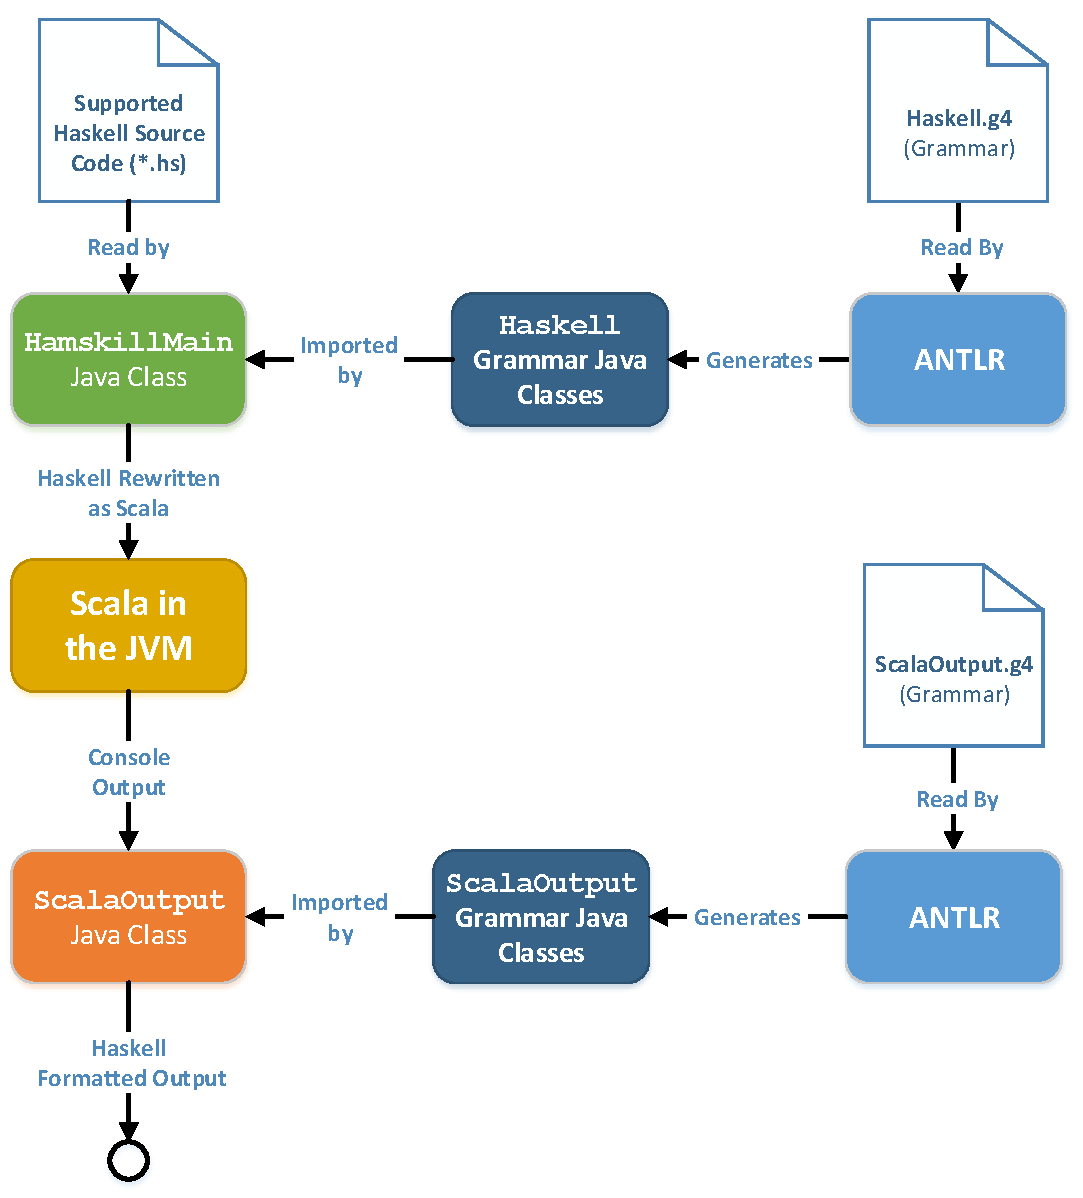
\includegraphics[width=1.0\textwidth]{images/cs252_project_diagram_cropped.pdf}
	\caption{HamSkill Project Architecture}
\end{figure}\label{fig:hamskillArchitecture}

The following subsections describe each of the components of this architecture.

\subsection{ANTLR}

ANTLR (\underline{AN}other \underline{T}ool for \underline{L}anguage \underline{R}ecognition) is an adaptive left-to-right, left-most deriviation (LL(*)) lexer and parser written in the Java programming language.  ANTLR's primary function is to read, parse, and process structured text (e.g. Haskell code) \cite{antlrDefinitiveReference}.  

\subsection{ANTLR Version 4 Grammar}

A grammar is a formal description of language; it is based off the concept of a context-free grammar in formal automata theory.  ANTLR version 4 (v4) grammar files (denoted by the file extension \emph{.g4}) explicitly define the how ANTLR will parse the structured text.  The grammar file may contain token definitions (which always start with a capital letter) and/or parser rules (which always start with a lowercase letter).  The tokens are groups of characters that form a single object; the parser then uses these tokens to recognize sentence structure within the document.

Two separate grammars are required for this project.  They are described in the following two subsections.

\subsubsection{Haskell Grammar}

\subsubsection{ScalaOutput Grammar}

\subsection{ANTLR Classes}

Programs that use ANTLR do not operate directly on the grammar.  Rather, the grammar is compiled by ANTLR into a set of class files; as such, given a grammar \emph{GrammarName.g4}, the following Java files would be created

\begin{itemize}
	\item \emph{GrammarName}Lexer.java - This class is the the lexer definition for the input grammar file.  It also extends ANTLR's base Lexer class.
	
	\item \emph{GrammarName}Parser.java - Each rule in the original grammar constitutes a method in this class; it forms the parser class definition for the input grammar file.
	
	\item \emph{GrammarName}.tokens - Assigns a token type (e.g. integer, identifier, floating point number etc.) to each token in the input grammar file.
	
	\item \emph{GrammarName}Listener.java \& \emph{GrammarName}BaseListener.java - ANTLR builds applies the grammar to a text input to build an Abstract Syntax Tree (AST).  While walking the tree, ANTLR fires events that can be captured by a listener\cite{antlrDefinitiveReference}.
\end{itemize}



\subsection{JVM-Supported Programming Language}

When selecting the implementation language, my criteria were: runnable in Java, and maximum similarity to Haskell.  I initially considered Python (via Jython) due to its higher order function support and concise style.  

In the end, I selected Scala for this project due to its syntax being more alignable to that of Haskell; an example of this is Scala's support for a function-based pattern matching style.  What is more, critical aspects of Haskell (e.g. lazy evaluation, immutability of objects, etc.) have parallels in Scala.  One major disadvantage of this decision is that Scala has a much weaker type inference system than Haskell or Python.  An example of this is described in section \ref{partiallyAppliedFunctions}.  

While it is my expectation that a fuller implementation of Haskell may be more achievable in Python, it would require substantially more effort to implement the functional programming aspects of Haskell that Scala comes with out of the box.  In the end, when doing a programming language conversion, it is exceptionally unlikely that the destination language will perfectly support all aspects of the source language.  As such, some degree of compromise is required which is why \emph{HamSkill} is only a dialect of Haskell.


\subsection{Immutability in Scala}\label{sec:immutabilityScala}

One of the key features of Haskell that allows it to achieve referential transparency is the immutability of data.  While it would be possible to develop an infrastructure in a language like Python to assure immutability, it is an encumbrance.  In cases such as this, it is almost always better to take advantage of a language's native features when possible.  In Scala, the {\tt val} construct ensure the immutability of an object without any user intervention.  For example, the code in figure~\ref{fig:scalaValConstruct} would raise a runtime error since it is trying to change the value of immutable data.

\begin{figure}[H]
\begin{mdframed}
\begin{lstlisting}[language=Scala]
val x = 5
x = 3
\end{lstlisting}
\end{mdframed}
\caption{Declaring Immutable Data in Scala}\label{fig:scalaValConstruct}
\end{figure}

\subsection{Lazy Evaluation}\label{sec:lazyEvaluationScala}

Another important aspect of Haskell is that it supports lazy evaluation.  This entails that data's value is not calculated until it is not needed.  Figure \ref{fig:lazyImmutabilityInScala} is an example of lazy evaluation with Scala as when this code is run, it will print a negative elapsed time (which is clearly not correct).

\begin{figure}[H]
\begin{mdframed}
\begin{lstlisting}[language=Scala]
def lazyTime(){
  lazy val t1 = System.nanoTime()
  val t2 = System.nanoTime()
  Thread.sleep(1000)
  println("Elapsed time is " + (t2-t1)/1000000 + "ms")
}
\end{lstlisting}
\end{mdframed}
\caption{Lazy, Immutable Code in Scala}\label{fig:lazyImmutabilityInScala}
\end{figure}

Scala also supports ``call-by-name" to achieve laziness of function parameters.  However, this feature is not truly lazy as it will recalculate the value each time the parameter is used in the function.  This limitation often degrades the overall the performance; for this reason, I do not plan to implement laziness in \emph{HamSkill} across functions.

\subsection{Supported Types}

\emph{HamSkill} will only support a select subset of Haskell's available types.  The list of planned types are: {\tt Bool}, {\tt Integer} (i.e. bounded), and {\tt List} (currently only finite lists are planned, but that may change depending on the complexity of the implementation).

While implementing floating point numbers would not add substantial complexity at a basic level, ensuring that the floating point behavior of \emph{HamSkill} (i.e. Scala) and Haskell are identical is beyond the scope of this project.

\subsection{From {\tt show} to {\tt toString}}

The function in Haskell to convert data to string is ``{\tt show}". In contrast, the syntax in Scala to convert an object (e.g. ``x") to a string is ``{\tt x.toString()}".  Due to this, the ANTLR parser will need to be able to convert a prefix function to an object method call.

\subsection{Nested Function Calls}\label{sec:nestedFunctionCalls}

Imperative languages (e.g. Java) are generally more verbose than functional languages; Haskell is no exception to this.  Conciseness introduces significant challenges when writing a parser as the contextual information is reduced.  For example, figure \ref{fig:addTwoNumbersHaskell} is a simple line of Haskell code that prints to the screen the result of a function ``{\tt addTwoNumbs}" that takes two integers (e.g. ``{\tt x}" and ``{\tt y}") and sums them. 

\begin{figure}[H]
\begin{mdframed}
\begin{lstlisting}[language=Haskell]
putStrLn $ show $ addTwoNumbs x y
\end{lstlisting}
\end{mdframed}
\caption{Simple Function Call in \textbf{Haskell}}\label{fig:addTwoNumbersHaskell}
\end{figure}

Similar code in Java is shown in figure \ref{fig:addTwoNumbersJava}

\begin{figure}[H]
\begin{mdframed}
\begin{lstlisting}[language=Java]
System.out.println( addTwoNumbs(x, y) ) ;
\end{lstlisting}
\end{mdframed}
\caption{Simple Function Call in \textbf{Java}}\label{fig:addTwoNumbersJava}
\end{figure}

The Java syntax explicitly shows that {\tt addTwoInts} is a function since the parameters are inside parentheses and are comma separated.  To simplify the parsing for this in Haskell, the \emph{HamSkill} dialect will require function arguments to be succeeded by double parentheses ``{\tt ((}" and ``{\tt ))}".  Figure \ref{fig:addTwoNumbersHamSkill} shows the \emph{HamSkill} version of the Haskell code in figure \ref{fig:addTwoNumbersHamSkill}.

\begin{figure}[H]
\begin{mdframed}
\begin{lstlisting}[language=Haskell]
putStrLn $ show $ addTwoInts ((x y))
\end{lstlisting}
\end{mdframed}
\caption{Simple Function Call in \textbf{\emph{HamSkill}}}\label{fig:addTwoNumbersHamSkill}
\end{figure}

\subsection{Defining Scope and Scala Object Name via {\tt module}}

A program in Haskell is composed of a set of ``{\tt module}" files.  The ``{\tt module}" keyword is used to  scope of functions (e.g. {\tt public} or {\tt private}) as well as for defining an abstract data type \cite{haskellModule}.  In \emph{HamSkill}, I will use the Haskell module to define whether the Scala methods are private (since by default functions are {\tt public}) as well as the name of the Scala object.

\subsection{Partially Applied Functions}\label{sec:partiallyAppliedFunctions}

Haskell supports partially applied functions.  Figure \ref{fig:addFiveHaskell} shows the {\tt addTwoInts} function with a single argument (i.e. ``{\tt 5}") being stored in a variable ``{\tt addFive}".  

\begin{figure}[H]
\begin{mdframed}
\begin{lstlisting}[language=Haskell]
let addFive = addTwoInts 5
\end{lstlisting}
\end{mdframed}
\caption{Partially Applied addTwoInts Function in \textbf{Haskell}}\label{fig:addFiveHaskell}
\end{figure}

Partially applied functions in Scala have advantages and disadvantages in comparison to Haskell.  One of these disadvantages is evident when figures \ref{fig:addFiveHaskell} and \ref{fig:addFiveScala} are compared.  Note that the Scala function requires an underscore ("\_") for each missing argument as well as the type for that argument.  This makes converting Haskell code to Scala problematic as the function prototype must be fixed and known at conversion time.  

\begin{figure}[H]
\begin{mdframed}
\begin{lstlisting}[language=Scala]
val addFive = addTwoInts(5, _: Int)
\end{lstlisting}
\end{mdframed}
\caption{Partially Applied {\tt addTwoInts} Function in \textbf{Scala}}\label{fig:addFiveScala}
\end{figure}

To simplify this, \emph{HamSkill} will require that any partially defined functions are declared in the same file/module.  I will investigate using a predefined list of functions, but this may not be feasible or support will be very limited due to the requirement to define the parameter type.  What is more, partially applied functions will use need to use the "double parentheses style" described in section \ref{sec:nestedFunctionCalls}.

\subsection{Higher Order Function Support}\label{sec:higherOrderFunctions}

Scala and Haskell are both functional programming languages; one important consequence of this is that both support higher order functions.  \emph{HamSkill} will support functions as input parameters to functions.  If time allows, I will also investigate the ability to return functions from functions.  The extent to which this is supported will be dependent on the extent to which partially applied functions are supported as defined in section \ref{partiallyAppliedFunctions}.

\subsection{Haskell Lambda Function to Scala Anonymous Functions}\label{sec:lambdaAnonymousFunctions}

There is significant similarity between a Lamda function in Haskell and an anonymous function in Scala.  One primary difference is that Scala requires the developer to specify the types of the parameters in the anonymous function while Scala does not. For this project, I will implement support for anonymous functions either as parameters to other functions or for support for an operation such as folding or filtering a list. 

\subsection{Maybe Monad Support}

\section{Test Bench}

\subsection{Implementation}

\pagebreak
\bibliographystyle{plainurl}
\bibliography{final_report_biblio}

\end{document}
